\chapter{Results}
\epigraph{The first law of thermodynamics says that work cannot be destroyed. We who use computers know better.}{A frustrated Ph.D. candidate}

\section{The Gang of Four}

Four new periodic orbits P85, P60, P32 and P8 (\refFigsss{fig:p85}{fig:p60}{fig:p32}{fig:p8}), also known as the Gang of Four, have been found, with properties that are summarized in \refTab{tab:summary}.  I was unable to find any \ecs\ in the fully unconstrained phase space. 

\begin{table}[h!]
\caption{A summary of relevant information regarding the Gang of Four. All of these results are presented at $\ReN = 400$, in the Hamilton-Kim-Waleffe cell\rf{Hamilton1995} with $(L_x,L_z) = (5.51157, 3.76239)$, and grid discretization $(N_x,N_y,N_z)= (48,33,48)$. The label for each orbit is based on its period, which experience shows uniquely defines an orbit. The phase velocities $v_x$ and $v_z$ are in terms of fraction of cell length per period. The largest Floquet exponent and number of unstable Floquet exponents are explained in a later section, as are the mean dissipation and energy input. The symmetry isotropy subgroup of each orbit is also provided. }   \label{tab:summary}
\begin{center}
\begin{tabular}{| r |  c | c | c | c | c | c | c | l |}
\toprule
Label & $T$ & $v_x$ & $v_z$ &  $\lambda_{\textrm{max}}$ & $\#\ \lambda_{\textrm{unstable}}$ & $\bar{D}/\bar{I}$&  Symmetry \\
\midrule
P85 & 85.50 & 0 & 0 & 0.0427 & 6 &1.85 & S\\
\midrule
P60 & 60.86 & 0 & 0 & FIND IT&10 & 2.08 & S\\
\midrule
P32 & 32.00 & 0.5 & 0 &  $0.0200 + 0.0982\imath$ & 7& 1.98 &$S_x$\\
\midrule
P8 & 8.32 & 0 & $2.29\times 10^{-7}$ & $0.0998 - 0.2605 \imath$ &20& 4.00& $S_z$\\
\bottomrule
\end{tabular}
\end{center}
\end{table}
\subsection{Visualizations}   

Visualizing the behavior of fluids is in itself a time-honored discipline, especially when CFD is involved,\footnote{As the old joke goes, CFD really stands for {\bf C}olorful {\bf F}luid {\bf D}ynamics.} and well chosen visualization schemes can be, in and of themselves, an excellent tool for interpreting and analyzing data. Here, we use two main visualization methods.
\subsubsection{Orthographic Projection}
\refFigsss{fig:p85}{fig:p60}{fig:p32}{fig:p8} are all examples of the first visualization method -- the {\bf orthographic projection} (OP)\rf{Gibson2008}. The OP is constructed by piecing together several representative 2D slices of the state's velocity field -- each of the periodic boundaries, and the mid-plane, and is colored to represent the magnitude and direction of streamwise velocity. The OP allows us to visually interrogate the structure of the state, which can be extremely useful -- for example, it is clear purely from visual interrogation that \refFig{fig:p8} is less ordered than \refFig{fig:p85}. However, the OP cannot deliver much more than this -- for example, it cannot easily tell us much about the differences between the orbits of, say, P8 and P85. For this reason, we use the second, more useful visualization method - the state space projection\rf{Gibson2008}.
\begin{figure}
\centerline{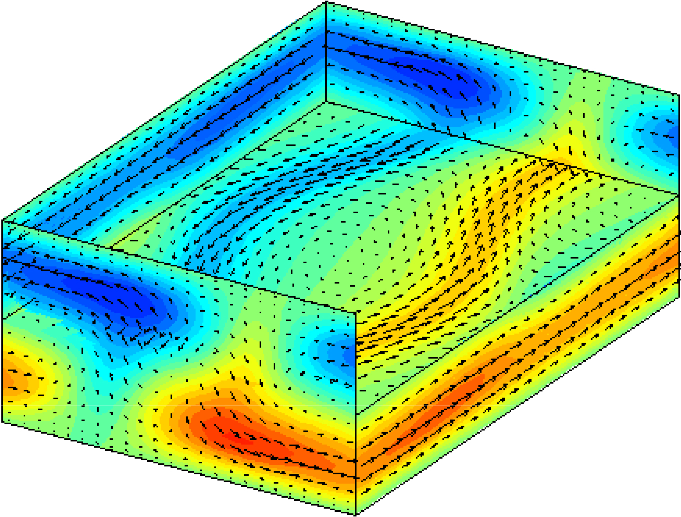
\includegraphics[width=\textwidth]{p85noBase.pdf}}
\caption{OP of P85. P85 is a fully symmetric orbit with period 85.50 in the HKW cell at $\ReN=400$. Note the extreme symmetry of the prominent streaks visible in the mid-plane. The velocity field pictured here is the turbulent perturbation only; the laminar flow has been subtracted away.{Available at {\tt https://youtu.be/r6ac1b54vDk}}}\label{fig:p85}
\end{figure}

\begin{figure}
\centerline{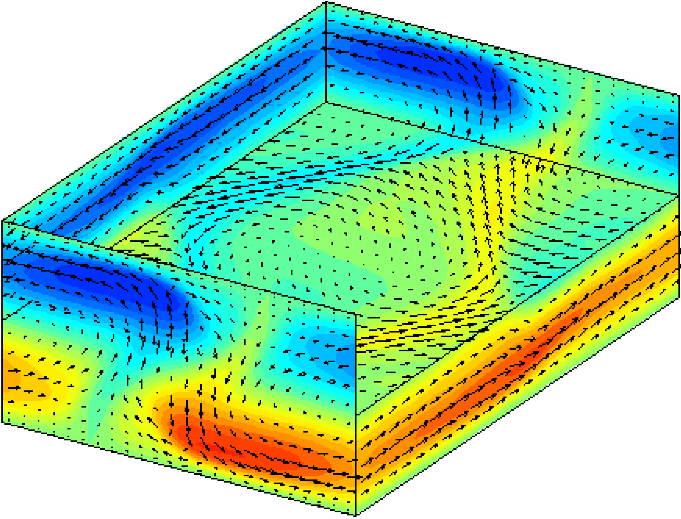
\includegraphics[width=\textwidth]{p60noBase.pdf}}
\caption{OP of P60. P60 is another fully symmetric orbit with period 60.86 in the HKW cell with $\ReN = 400$. While it displays an ellipsoid streak structure similar to P85, the energy of these streaks is lower.The velocity field pictured here is the turbulent perturbation only; the laminar flow has been subtracted away.{Available at {\tt https://www.youtube.com/watch?v=ulyMrSfxW5U}}}\label{fig:p60}
\end{figure}


\begin{figure}
\centerline{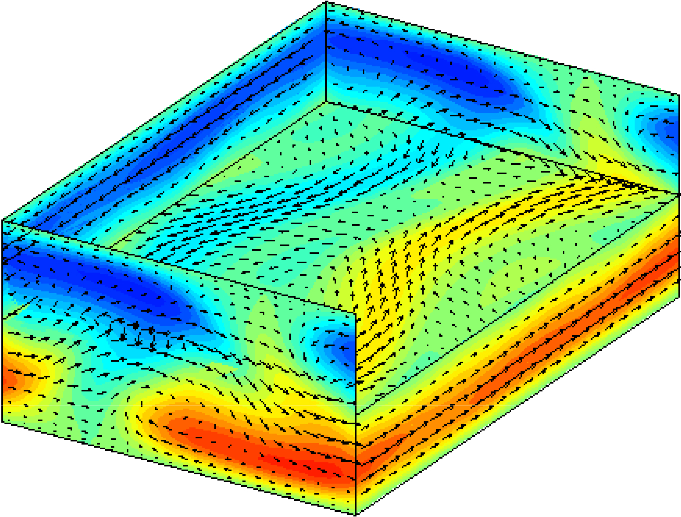
\includegraphics[width=\textwidth]{p32noBase.pdf}}
\caption{OP of P32. P32 is a streamwise asymmetric periodic orbit fixed by the symmetry group $S_z$, which is functionally a mirror symmetry about the streamwise axis. In the HKW cell at $\ReN=400$, the period is 32.00, and the streamwise relative velocity is $-0.5$ cell lengths per period.The velocity field pictured here is the turbulent perturbation only; the laminar flow has been subtracted away. Available at {\tt https://www.youtube.com/watch?v=qDGbxX50bKY}}\label{fig:p32}
\end{figure}


\begin{figure}
\centerline{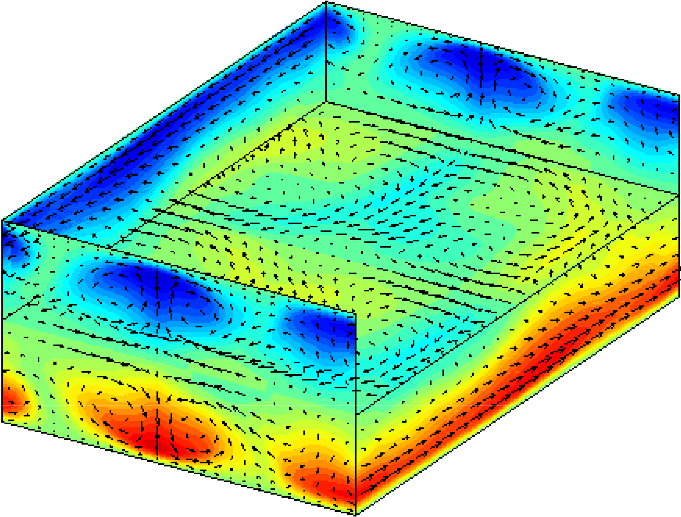
\includegraphics[width=\textwidth]{p8noBase.pdf}}
\caption{OP of P8. P8 is a spanwise asymmetric periodic orbit fixed by the symmetry group $S_x$, which is functionally a rotation by $\pi$ about the spanwise axis. In the HKW cell at $\ReN = 400$, the period is 8.32, and the spanwise relative velocity is $2.29\times 10^{-7}$ cell lengths per period. This number may seem low, but if it is not accounted for, the NKH solver cannot converge. P8 also has a rather short period, almost an order of magnitude shorter than most orbits recorded in the database at {\tt channelflow.org}. Since the Arnoldi iteration has a time cost that scales linearly with the period, P8 has been the least computationally demanding period orbit to analyze. The velocity field pictured here is the turbulent perturbation only; the laminar flow has been subtracted away. Available at {\tt https://youtu.be/-ad0U55T39w}}\label{fig:p8}
\end{figure}



\begin{figure}[h]
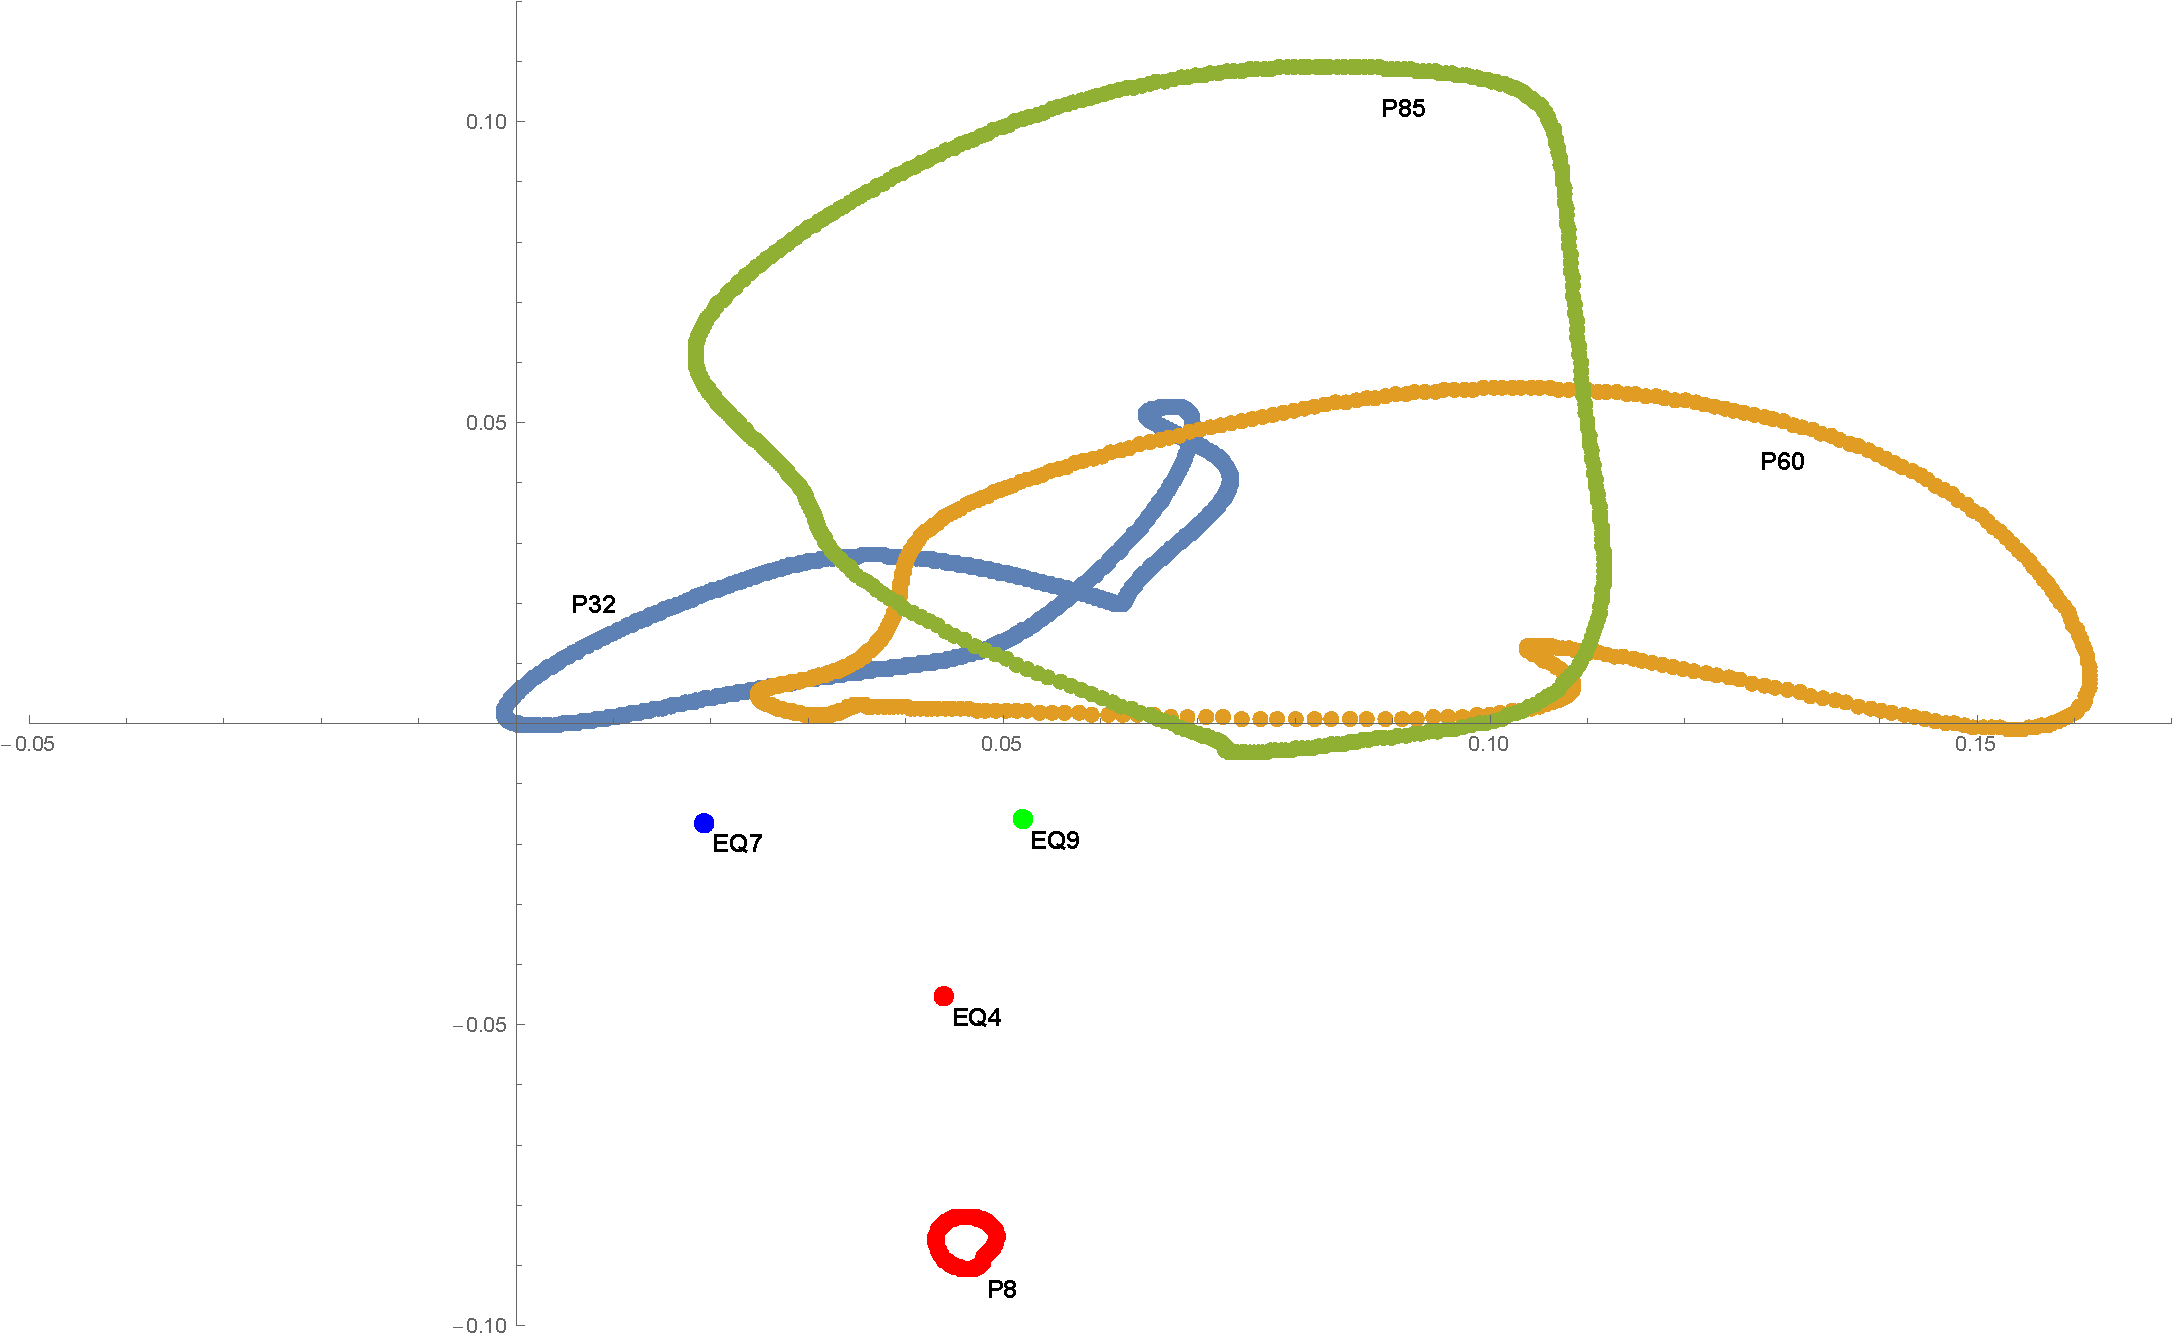
\includegraphics[width=\textwidth]{PeriodicOrbitPO412}
\caption{2D state space projection of the Gang of Four and some reference equilibria. The basis vectors for the projection were constructed by orthonormalizing the initial states of each of the periodic orbits. This results in a 4D state space projection, of which we can take 2D slices (of which there are 6), or 3D slices (of which there are 4). The equilibria are fully symmetric, and were found by Halcrow\rf{Halcrow2008}. Notice that the P8 orbit is separated by the equilibria from P85, P60 and P32, a feature that holds true in the other 5 2D projections.}\label{fig:POStateSpace}
\end{figure}

\subsubsection{State Space Projection}
If we have a set of $k$ basis vectors $\Vector{q}_i$ that are orthonormal and span a subspace $\mathfrak{V}_k \subset \mathfrak{V}$ of dimension $k$, then the projection of a vector $\Vector{v} \in \mathfrak{V}$ onto $\mathfrak{V}_k$ is defined 
\begin{equation}
\Vector{v}_k = \sum{i = 1}{k}{c_i \Vector{q}_i},
\end{equation}
where $c_i = \Vector{v} \cdot \Vector{q}_i$. When $k$ is either 2 or 3, we can visualize the $n$-dimensional trajectory as a 2 or 3 dimensional trajectory instead. While we lose information in making this projection, we can still gain a great deal of valuable information about trajectories. Projecting the four periodic orbits in \refFigRange{fig:p85}{fig:p8} onto a basis constructed from orthonormalizing the initial conditions of each orbit results in the state space projection in \refFig{fig:POStateSpace}.\\

 The main issue with the state space projection method, however, is that a state must be {\bf congruent} to a basis to be projected onto it - that is, both the box length and grid discretization must be the same for both the state and the projection basis. Many previous investigations\rf{Halcrow2008,Gibson2008} have results in the W03 cell, where $(L_x,L_z) = (5.51157,2.51327)$, with corresponding state space projections. In order to compare to these results, I attempted to use \refAlg{alg:parCont} to continue the four periodic orbits into the W03 cell, which leads me to the next important result.

\section{Spanwise Continuation}

When \refAlg{alg:parCont} was used to continue P8 down to the W03 cell, the data presented in \refFig{fig:LZBif} was produced.  Initially, the continuation algorithm decreases $L_z$ and increases $T$, but at $L_z \approx 2.8$, the algorithm reverses itself, decreasing $T$ and increasing $L_z$, until $L_z \approx 2.95$, when the algorithm resumes decreasing $L_z$ and increasing $T$. Since we expect that the period of an orbit ought to uniquely define the orbit,\footnote{We generally assume that if two solutions have differing periods, they are distinct, which may seem reasonable - but holes in such a simple criterion are evident almost immediately. For example, two `distinct' orbits with periods $T_1$ and $T_2$ may in fact be the same orbit, with period $|T_2-T_1|$, that has simply repeated more times for one orbit than for the other. This hole can be plugged by any number of methods, most easiest by simply calculating $||\Vector{u}_1(t) - \Vector{u}_2||$ over the entire period. If the norm is never small, then the orbits are distinct. }  the existence of multiple, distinct orbits for $2.8 \leq L_z \leq 2.96$ hints at a bifurcation. 
\begin{figure}[t]
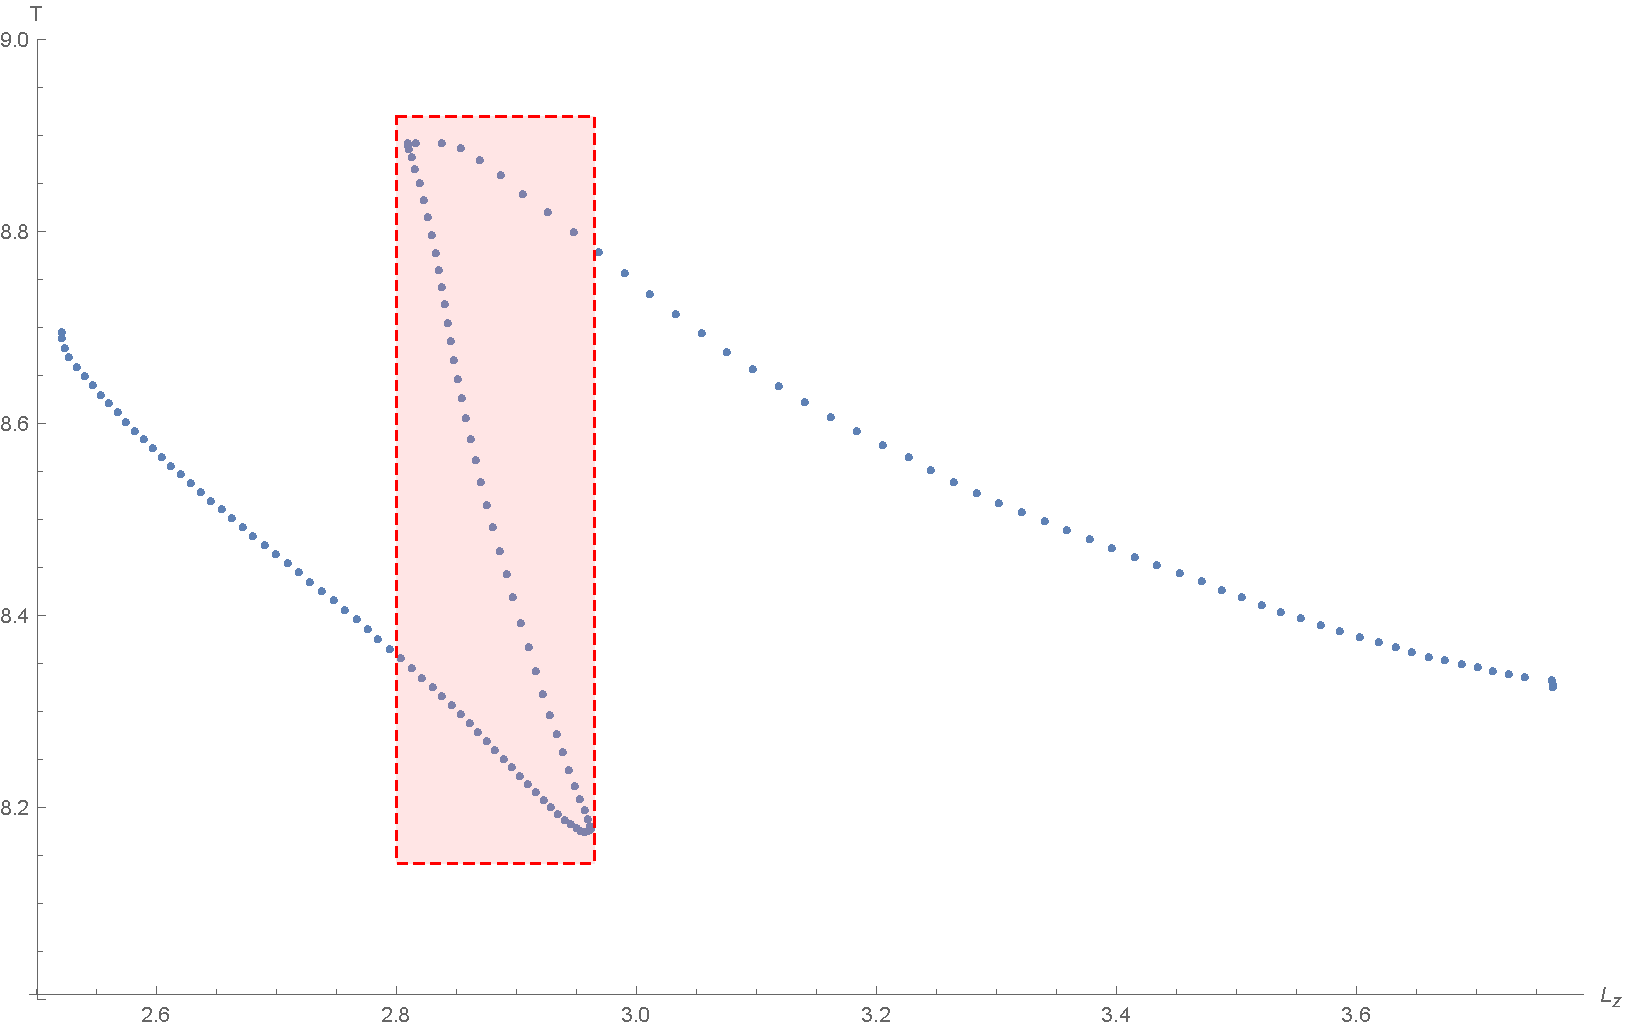
\includegraphics[width=\textwidth]{TLzBD}
\caption{Period as a function of spanwise cell length for P8. The data can be sectioned into three distinct parts. First, the {\bf upper branch} (blue circles), which is the path that the continuation algorithm initially follows in parameter space. Second, the {\bf transition branch} (green diamonds), which occurs after the {\bf first turning point} (red, dashed circle). Third, the {\bf lower branch} (orange rectangles), after the {\bf second turning point} (purple, solid circle). Within the marked rectangular region, multiple distinct solutions exist for the same cell length, hinting at a bifurcation.}\label{fig:LZBif}
\end{figure}
\begin{figure}[t]
\includegraphics[width=\textwidth]{phasePortraitTransition}
\caption{Phase portrait of the Van Der Pol oscillator and its Hopf bifurcation, with trajectories in white. (a), for negative values of the bifurcation parameter, the single periodic orbit is unstable, so an initial condition that begins near the orbit spirals away from it. (b), when the bifurcation parameter is zero, there is no periodic orbit. (c), for positive values of the bifurcation parameter, the periodic orbit is stable, and initial conditions are attracted into the orbit.}\label{fig:phasePortrait}
\end{figure}
 The similarity of \refFig{fig:LZBif} to \refFig{fig:bifurcations} is striking, and led me to suspect the possibility that P8 undergoes some form of bifurcation at $L_z \approx 2.8$ and $L_z \approx 2.95$. However, \refAlg{alg:parCont} relaxes the convergence criteria to $10^{10}$ to speed up the parametric continuation process, and as a result, may have found artificial solutions, so I verified the existence of multiple distinct solutions for $L_z = 2.925$ and $(N_x,N_y,N_z) = (62,53,62)$ to $10^{-13}$. However, this in and of itself does not necessarily prove that a bifurcation exists -- for example, the continuation algorithm may have simply found \emph{another} periodic orbit's trajectory and hopped onto that. When a bifurcation occurs, the qualitative behavior of solutions pre and post-bifurcation tend to be markedly different. For low-dimensional systems, this is easy to evaluate, since one can visually identify changes in the phase space, as in \refFig{fig:phasePortrait}. For higher-dimensional systems, such an approach is not feasible. 

\subsection{Linear Stability Analysis}\label{sec:LSA}

We can instead turn to {\bf linear stability analysis}. If $\Vector{u}$ is a periodic orbit with period $T$, then for a small perturbation ${\bf \textrm{d}}\Vector{u}$, 
\begin{equation}\label{eq:linearStable}
 f_T(\Vector{u} + {\bf \textrm{d}}\Vector{u}) - \Vector{u} =  f_T(\Vector{u}) - \Vector{u} + \mathbb{J}_{T,\Vector{u}}{\bf \textrm{d}}\Vector{u} =  \mathbb{J}_{T,\Vector{u}}{\bf \textrm{d}}\Vector{u},
\end{equation} 
where $ \mathbb{J}_{T,\Vector{u}}$ is the Jacobian of the Navier-Stokes forward-time map evaluated at $\Vector{u}$. The stability of the orbit is determined by how  ${\bf \textrm{d}}\Vector{u}$ changes over time - if it shrinks, then the orbit is stable, but if it grows, it is unstable. Writing  ${\bf \textrm{d}}\Vector{u}$ as a linear combination of the eigenvectors $\Vector{v}_i$ of  $ \mathbb{J}_{T,\Vector{u}}$, the right-hand side of \eqref{eq:linearStable} becomes
\begin{equation}\label{eq:oneOrbit}
 \mathbb{J}_{T,\Vector{u}}{\bf \textrm{d}}\Vector{u} =  \mathbb{J}_{T,\Vector{u}}\sum{i = 1}{n}{c_i\Vector{v}_i} = \sum{i = 1}{n}{c_i\lambda_i\Vector{v}_i},
\end{equation}  
where the $\lambda_i$ are the corresponding eigenvalues, known as the {\bf Floquet exponents}, whose real parts measure the exponential rate of decay or growth of the corresponding eigenvector.\footnote{The real parts are known as the {\bf Lyapunov exponents}. The imaginary part contributes only to the oscillatory behavior.}   From this definition, it is clear that the periodic orbit can only be stable against infinitesimal perturbations if $\textrm{Re}[\lambda_i]  \leq 0~\forall~i$, and unstable otherwise. The eigenvalues for the Navier-Stokes forward-time map can be calculated by \refAlg{alg:Arnoldi}. The eigenvalues of P8 in the HKW cell at $\ReN=400$ are shown in \refFig{fig:P8Eigenvals}

\begin{figure}[h]
\includegraphics[width=\textwidth]{P8Eigenvals}
\caption{All 20 unstable eigenvalues, and the 80 largest stable or marginal $(|\lambda| << 1)$ eigenvalues of P8, in the HKW cell at $\ReN=400$. Note that the eigenvalues come in conjugate pairs. Since there are eigenvalues with positive real parts, the periodic orbit is unstable, as expected. Note that since the Jacobian likely has full rank, and likely also has no repeating nonzero eigenvalues, there are several orders of magnitude more stable eigenvalues than there are unstable. Since the Arnoldi iteration will find the larger eigenvalues first, all the unstable eigenvalues are shown, whereas only the weakly stable eigenvalues are calculated.}\label{fig:P8Eigenvals}
\end{figure}

In general, we would expect that as the control parameter changes, the Lyapunov exponents would also. In particular, if a change in the control parameter resulted in the Lyapunov exponent changing sign, the qualitative behavior of the periodic orbit would change, resulting in a bifurcation. Applying the Arnoldi iteration to the states near the turning points of \refFig{fig:LZBif} results in \refFig{fig:P8FirstBifurcation} and \refFig{fig:P8SecondBifurcation}. 
\clearpage
 \refFigs{fig:P8FirstBifurcation}{fig:P8SecondBifurcation} have a set of eigenvalues that switch sign at $L_z$ values that are reasonably consistent with turning point data from \refFig{fig:LZBif}. It therefore seems likely that these turning points do in fact correspond to bifurcations. Qualitative differences between the upper and transition branch are also apparent from observations of movies of the periodic orbit.\footnote{Available at {\tt https://youtu.be/JDzQfjx5Cmg}} From the video, it appears that the upper branch has more energy concentrated in the streaks than the transition branch, which in turn appears to have more energy in the mid-plane. \\

\begin{figure}[t]
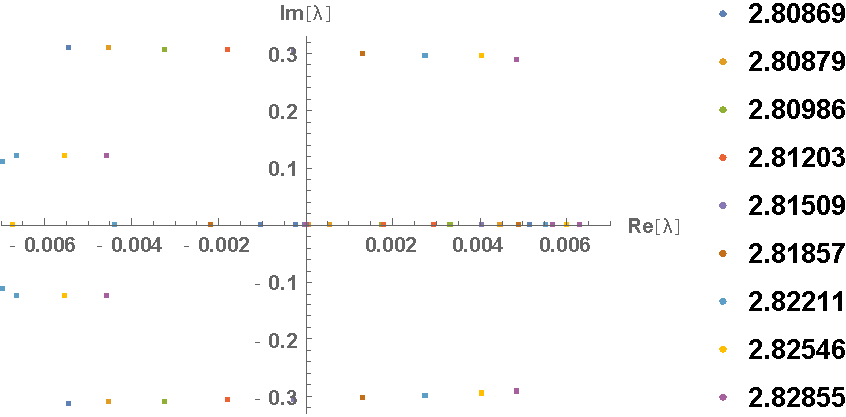
\includegraphics[width=\textwidth]{P8FirstBifurcation}
\caption{Eigenvalues of P8 as a function of $L_z$ at the first turning point. Of interest are the eigenvalues with imaginary part $\approx \pm 0.3$. From left to right, the eigenvalues of $L_z = 2.8088757,$ $2.8087205,$ $2.8087115,$ $2.8096095,$ $2.8116723,$ $2.8147572,$ $2.8184122,$ $2.8221628$ and $2.8257047$. The real part of the eigenvalue likely switches sign at some $L_z \in [2.81476,2.81841]$, compared to the first turning point, which likely occurs for $L_z \in [2.8087205, 2.8096095]$  }\label{fig:P8FirstBifurcation}
\end{figure}


\begin{figure}[h]
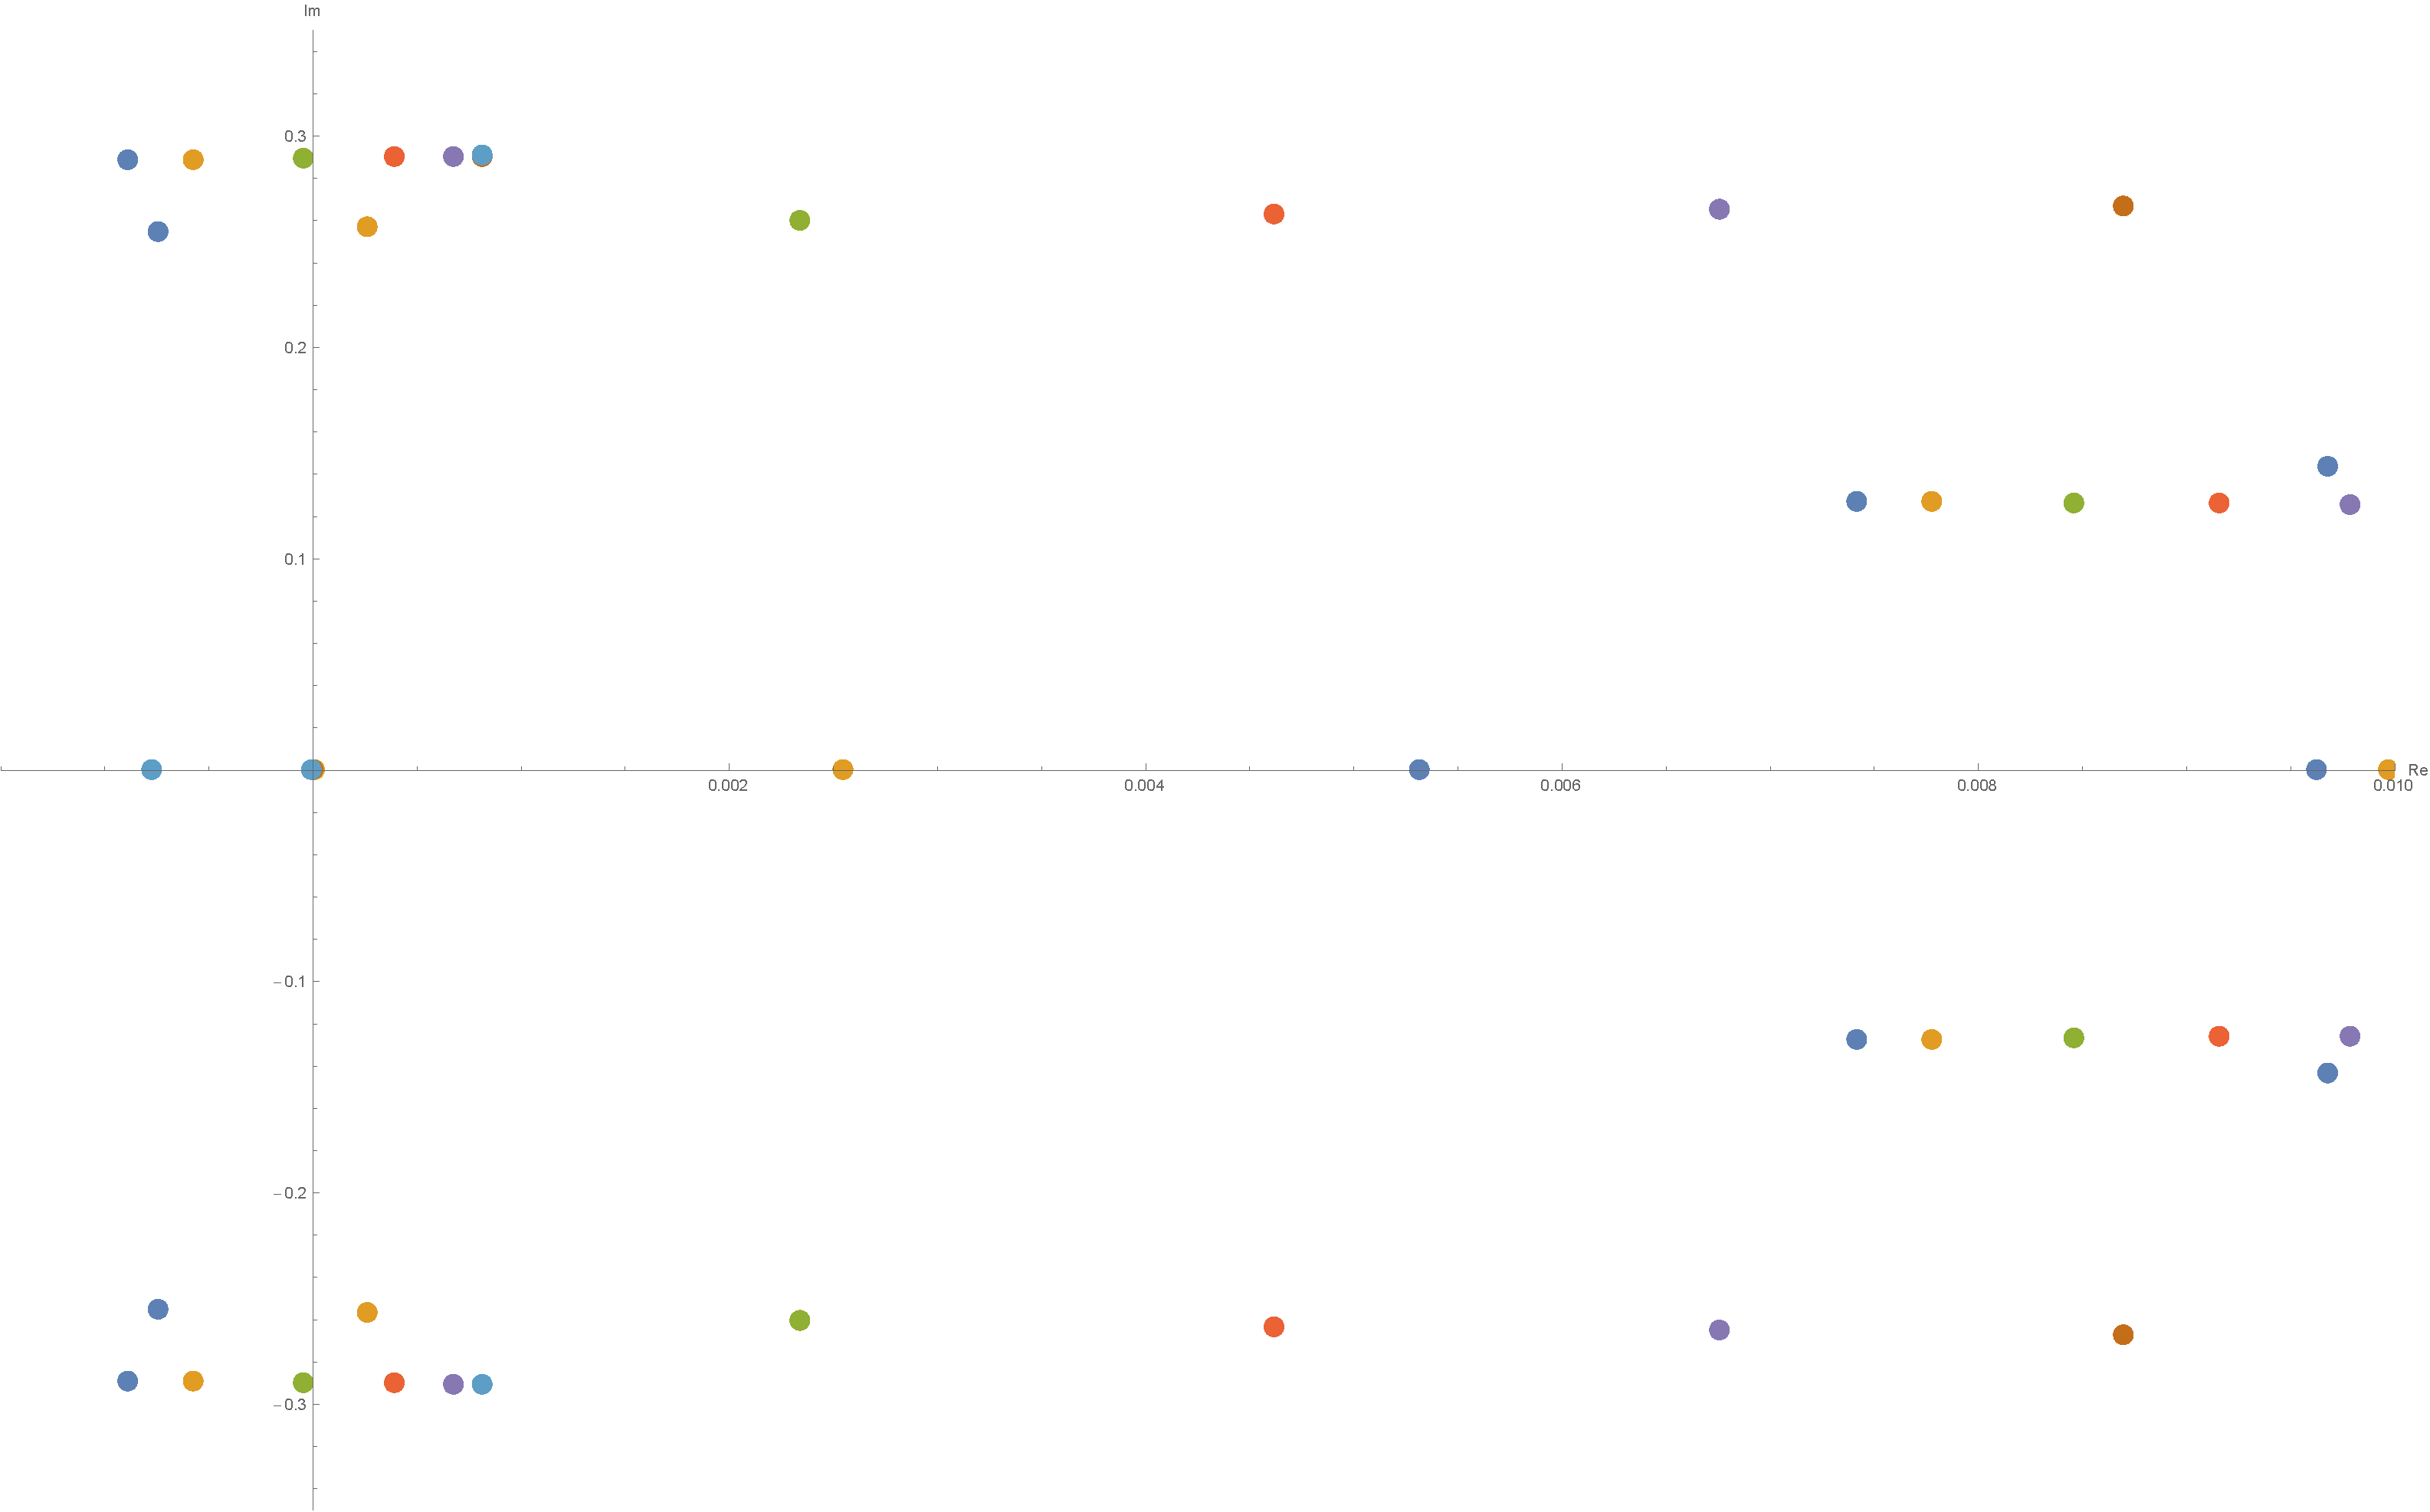
\includegraphics[width=\textwidth]{P8SecondBifurcation}
\caption{Eigenvalues of P8 as a function of $L_z$ at the second turning point. From left to right, the eigenvalues of  $L_z =  2.9612911,$ $2.9614915,$ $2.961412,$ $2.9605641,$ $2.9589117,$ $2.9564639,$ and $2.9532518$. Two sets of eigenvalues have real parts that switch signs, at $L_z \in [2.961412,2.9605641]$ and $L_z \in [ 2.9612911,2.9614915]$. This is consistent with analysis of the turning point, which indicates that the bifurcation occurs for $L_z \in [ 2.9612911, 2.961412]$.}\label{fig:P8SecondBifurcation}
\end{figure}

\subsection{Return of the State Space}

Having used linear stability analysis to find the unstable eigenvector, we can use the state space projection to visualize the effect of a slight perturbation, as  in \refFig{fig:p8E1}. Here, we see the effect of a slight perturbation along the most unstable eigenvector $P8E1$, with eigenvalue $0.0998 - 0.2605 i$. Now \refFig{fig:p8E1} is noisy, and difficult to analyze. To deal with this, we can construct the {\bf Poincare section} of a trajectory. The Poincare section of a $k$ dimensional trajectory is constructed by keeping track of where the trajectory crosses a $k-1$ dimensional surface. The Poincare section for  $P8E1$, displayed in \refFig{fig:E1Poincare} displays the qualitative behavior we would expect for a complex eigenvalue - the real part is negative and the perturbation grows, the imaginary part is nonzero, and the perturbation spirals around the initial position. Even though the eigenvalue is only valid locally, we can still see that it approximately predicts the behavior of the trajectory - from the imaginary part of the eigenvalue, we can see that it ought to take approximately 25 time units for a full rotation in the Poincare section. \refFig{fig:E1Poincare} suggests that approximately 5 orbits have taken place for a full rotation in the Poincare section, each with periods that are approximately 8 time units. This does not agree exactly,\footnote{Or very well at all, especially since we've just come from having residuals on the order of $10^{-14}$} but one must remember that the Floquet exponents are a \emph{local} model of the orbit, and naturally become less precise the more the perturbation grows.\footnote{As a matter of fact, the pictured spiral is the last spiral the Poincare section trajectory executes, though the trajectory in the full space continues to look qualitatively similar to the original orbit for a long time.}   


\begin{figure}[h!]
\centerline{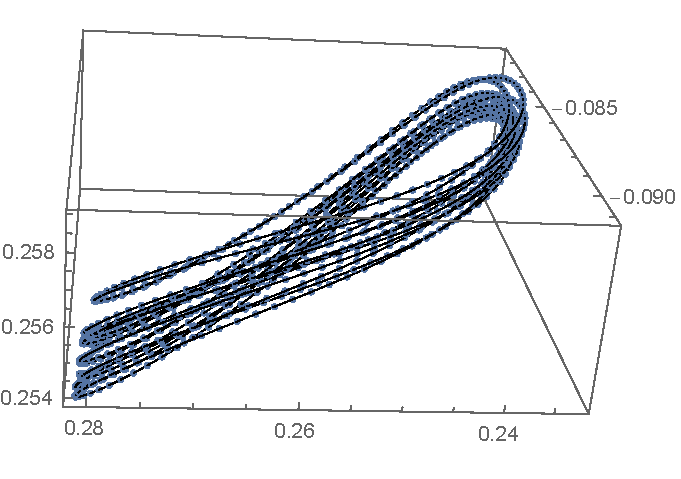
\includegraphics[scale=1]{E1Perturb}}
\caption{The trajectory of a slight perturbation along the most unstable eigenvector, projected onto a difference slice of the same basis as in \refFig{fig:POStateSpace}. Notice that it keeps the general shape of the orbit that spawned it, at least for short time spans.}\label{fig:p8E1}
\end{figure}

\begin{figure}[h!]
\centerline{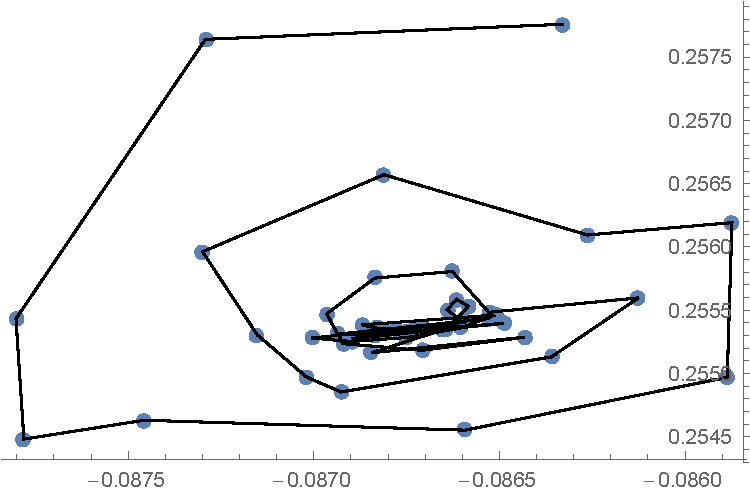
\includegraphics[scale = 0.9]{E1Poincare}}
\caption{Poincare section of \refFig{fig:p8E1}, defined by the surface $e_2 = 0.26$. Notice that the trajectory along the Poincare section spirals outwards, as we would expect for an unstable manifold with a complex eigenvalue.}\label{fig:E1Poincare}
\end{figure}

\section{Dissipation and Energy Input} 
  
\subsection{A New State Space}
While \refFig{fig:POStateSpace} seems to indicate that P8 is a special member of the Gang of Four -- an assertion which is backed up by the marked difference in the properties displayed in \refTab{tab:summary} -- the striking dissimilarty in \refFig{fig:POStateSpace} may be an artifact of the projection basis. To address this issue, we can also project onto the {\bf dissipation-energy input} plane, where the dissipation $D$ and energy input $I$ are defined
\begin{align}
D(t) = \frac{1}{L_xL_yL_z}\int{0}{L_x}{\int{0}{L_y}{\int{0}{L_z}{|\nabla\times\Vector{u}(t)|^2}{\textrm{d}z}}{\textrm{d}y}}{\textrm{d}x},\\
I(t)  = 1 + \frac{1}{2L_xL_z}\int{0}{L_x}{\int{0}{L_z}{\pder{1}{\Vector{u}_{y}}{y} |_{y=1}+\pder{1}{\Vector{u}_{y}}{y} |_{y=-1}}{\textrm{d}z}}{\textrm{d}x},
\end{align} 
resulting in \refFig{fig:DIGOF},\footnote{Note that for a periodic orbit, the mean dissipation and energy input need to be balanced, which explains why all observed solutions do not stray far away from the line $D(I) = I$.} which suggests that the distinctive features of P8 are likely not artificial.  

\begin{figure}[h]
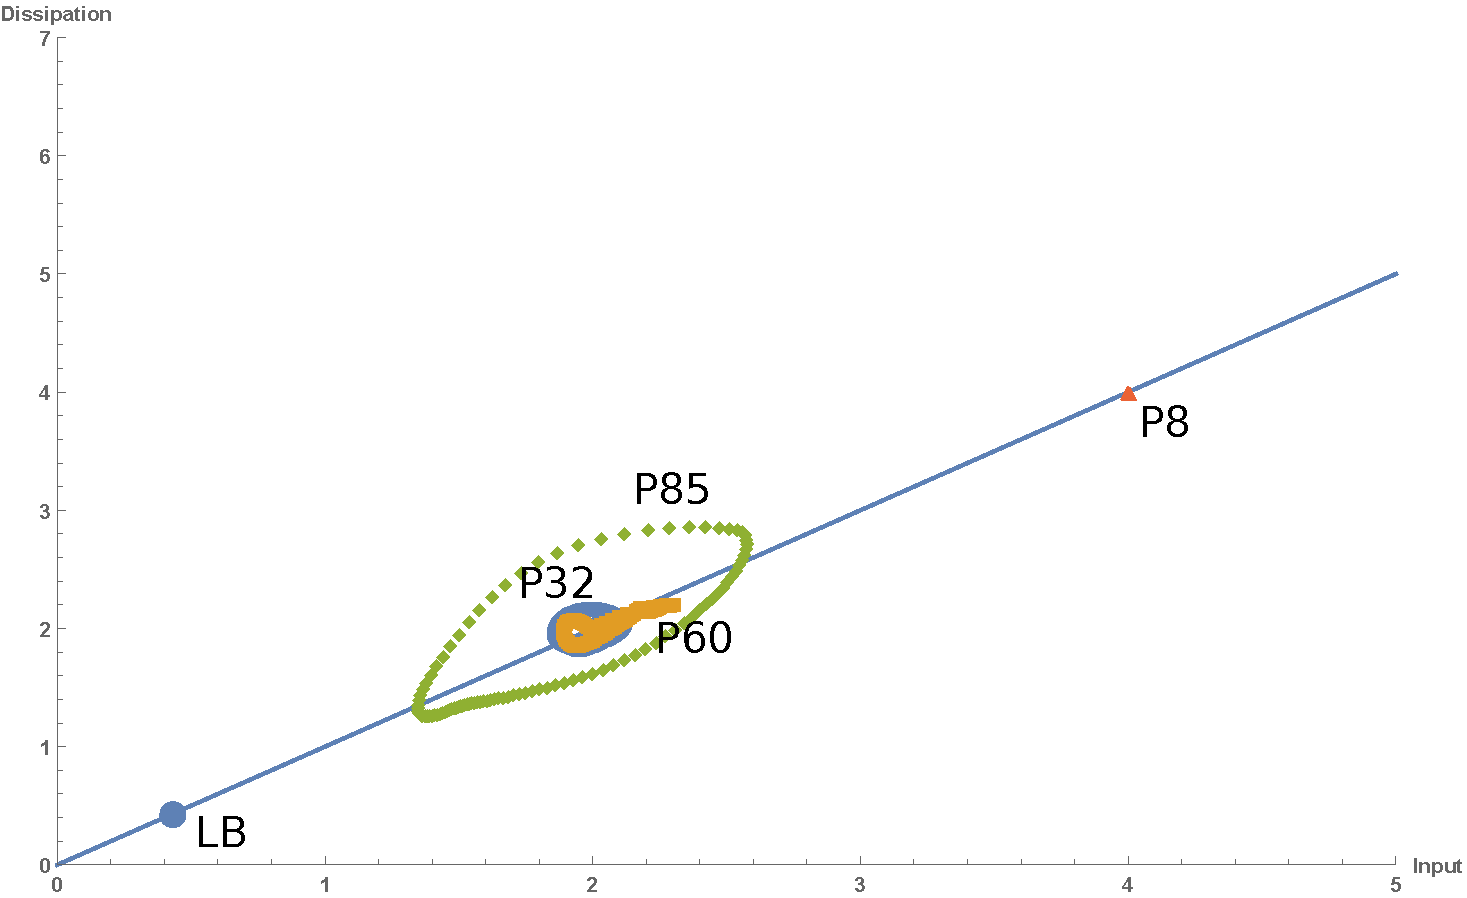
\includegraphics[width=\textwidth]{DIOG}
\caption{Dissipation versus energy input for the Gang of Four. While the lesser members of the Gang remain clustered towards a input/dissipation of 2, P8 stays at a dissipation/input of 4. Due to P8's low period, the fine details of its orbit cannot be discerned here. The separation observed in \refFig{fig:POStateSpace} is clearly reflected in this physically important projection.}\label{fig:DIGOF}
\end{figure}

\subsection{The Return of the Bifurcation}



Alas, at this point we cease our analysis, for all good things must come to and end. This analysis is by no means complete or comprehensive -- there is likely a great deal more to learn regarding the properties of symmetry broken periodic orbits, but due to time constraints, I will cut the analysis short here, and proceed to summarize the work of this thesis, and suggest avenues to research, moving forward. 
